% ─────────────────────────────────────────────────────────────────────────────
% Supplementary Material, SplitGuard-AD (Journal of Imaging Informatics in
% Medicine submission)
%
% This file bundles the supplementary sections referenced from the main
% manuscript and is compiled independently for the supplementary upload.
% ─────────────────────────────────────────────────────────────────────────────
\documentclass[11pt]{article}
\usepackage[utf8]{inputenc}
\usepackage[T1]{fontenc}
\usepackage{amsmath,amssymb}
\usepackage{booktabs}
\usepackage{array}   % >{...} column modifiers used by the moved tables
\usepackage{graphicx}
\usepackage{float}
\usepackage{xcolor}
\usepackage[margin=1in]{geometry}
\usepackage{hyperref}

\newcommand{\SGA}{\textsc{SplitGuard-AD}}
\newcommand{\ie}{\textit{i.e.},}
\newcommand{\eg}{\textit{e.g.},}
\newcommand{\etal}{\textit{et al.}}
\newcommand{\gap}[1]{#1}
\renewcommand{\thesection}{S\arabic{section}}
\renewcommand{\thetable}{S\arabic{table}}
\renewcommand{\thefigure}{S\arabic{figure}}
\renewcommand{\theequation}{S\arabic{equation}}

\title{Supplementary Material \\
\textsc{SplitGuard-AD}: Executable Leakage Auditing for Slice-Based
Alzheimer's Disease MRI Deep Learning Benchmarks}
\author{}
\date{}

% Numbers generated by scripts/gpu_postprocess.py.
% Generated by scripts/gpu_postprocess.py. Do not edit by hand.
% \pending marks a number whose run has not completed.
\providecommand{\pending}{\textbf{??}}
\newcommand{\TierOneRandomAUROC}{0.999}
\newcommand{\TierOneFilenameAUROC}{0.793}
\newcommand{\TierOneTrueAUROC}{0.766}
\newcommand{\TierOneGapTotal}{+0.233}
\newcommand{\TierOneGapCI}{[+0.191, +0.270]}
\newcommand{\TierOneGapFilename}{+0.206}
\newcommand{\TierOneGapResidual}{+0.027}
\newcommand{\TierOneShareFilename}{88.6}
\newcommand{\AdniRandomAUROC}{0.947}
\newcommand{\AdniSubjectAUROC}{0.837}
\newcommand{\AdniSafeAUROC}{0.829}
\newcommand{\AdniGapTotal}{+0.118}
\newcommand{\AdniGapCI}{[+0.096, +0.145]}
\newcommand{\AdniHierGap}{+0.118}
\newcommand{\AdniHierCI}{[+0.061, +0.181]}
\newcommand{\AdniGapExactKey}{+0.113}
\newcommand{\AdniDenseGap}{+0.146}
\newcommand{\AdniConvGap}{+0.142}
\newcommand{\AdniNoMtOneGap}{+0.128}
\newcommand{\AdniNoMtOneCI}{[+0.097, +0.159]}
\newcommand{\SizeBalancedGap}{+0.136}
\newcommand{\AdniSubjectPart}{0.110}
\newcommand{\AdniSubjectPartCI}{[+0.086, +0.139]}
\newcommand{\AdniMarginal}{0.008}
\newcommand{\AdniMarginalCI}{[-0.033, +0.042]}
\newcommand{\AdniConvMarginal}{-0.026}
\newcommand{\AdniArmSpread}{0.028}
\newcommand{\OasisRandomAUROC}{0.828}
\newcommand{\OasisSafeAUROC}{0.793}
\newcommand{\OasisGapTotal}{+0.035}
\newcommand{\OasisGapCI}{[+0.009, +0.064]}
\newcommand{\OasisDenseGap}{+0.048}
\newcommand{\VolGapTotal}{+0.235}
\newcommand{\VolGapCI}{[+0.174, +0.298]}
\newcommand{\ProbeLiftImage}{211.7}
\newcommand{\ProbeLiftSession}{204.8}
\newcommand{\ProvScanTenSubject}{35\%}
\newcommand{\ProvScanTenSafe}{18\%}
\newcommand{\ProvParticipantTenSubject}{36\%}
\newcommand{\ComposedTenSubject}{0.043}
\newcommand{\ComposedTenSafe}{0.022}
\newcommand{\ProvSubjectAUROCTen}{0.865}
\newcommand{\ProvSafeAUROCTen}{0.829}
\newcommand{\CardSens}{65.5\%}
\newcommand{\CardSpec}{81.0\%}
\newcommand{\CardBalAcc}{73.2\%}
\newcommand{\CardAUROC}{0.829}
\newcommand{\CardNTest}{165}
\newcommand{\CardPPVPop}{35.6\%}
\newcommand{\CardNPVPop}{93.6\%}
\newcommand{\CardPPVClinic}{83.2\%}
\newcommand{\CardNPVClinic}{62.1\%}
\newcommand{\GpuHours}{14.8}
\newcommand{\DoseSlope}{0.125}
\newcommand{\DoseAtZero}{0.823}
\newcommand{\DoseDenseAtZero}{0.861}
\newcommand{\DoseDenseSlope}{0.091}
\newcommand{\DoseAtOne}{0.948}
\newcommand{\AdniConvRandomAUROC}{0.957}
\newcommand{\AdniConvSafeAUROC}{0.815}
\newcommand{\DoseIntercept}{0.823}
\newcommand{\DoseRSq}{0.853}
\newcommand{\SensLeaky}{0.866}
\newcommand{\SensSafe}{0.535}
\newcommand{\MissedPerThousand}{45.7}
\newcommand{\AdniShareSubject}{93}


\begin{document}
\maketitle

% ═══════════════════════════════════════════════════════════════════════════
\section{Consolidated training hyperparameters}
\label{sm:hyperparams}
% ═══════════════════════════════════════════════════════════════════════════

Table~\ref{tab:sm_hyperparams} lists the full per-cohort training
configuration referenced in the main text.

\begin{table}[!ht]
\centering
\footnotesize
\caption{Consolidated training hyperparameters across the three
tiers and both backbones.}
\label{tab:sm_hyperparams}
\begin{tabular}{@{}p{3.2cm}p{3.3cm}p{3.3cm}p{4.3cm}@{}}
\toprule
Parameter & Kaggle & OASIS-1 & ADNI1 \\
\midrule
Backbones & ResNet-18; DenseNet-121 & ResNet-18; DenseNet-121 &
ResNet-18 primary; DenseNet-121 architecture arm \\
Initialisation & ImageNet & ImageNet & ImageNet \\
Input & $3\!\times\!224\!\times\!224$ & $3\!\times\!224\!\times\!224$ & $3\!\times\!224\!\times\!224$ \\
Normalisation & ImageNet mean/std & ImageNet mean/std & ImageNet mean/std \\
Augmentation & flip + $\pm 7^{\circ}$ & flip + $\pm 7^{\circ}$ & flip + $\pm 7^{\circ}$ \\
Epochs & 30 & 20 & 15 (all arms) \\
Optimiser & AdamW & AdamW & AdamW \\
Learning rate & $3\!\times\!10^{-4}$ & $3\!\times\!10^{-4}$ & $10^{-4}$ \\
LR schedule & Cosine anneal & Cosine anneal & Cosine anneal \\
Weight decay & $10^{-2}$ & $10^{-2}$ & $10^{-2}$ \\
Batch size & 32 & 32 & 16 \\
Loss & inverse-freq BCE & inverse-freq BCE & inverse-freq BCE \\
Seed array & $\{0,1,2,3,42\}$ & $\{0,1,2,3,42\}$ & $\{0,1,2,3,4\}$ \\
Backend & CUDA H100 & CUDA H100 & CUDA H100; RTX PRO 4500 \\
         &          &          & (dose-response matrix); \\
         &          &          & RTX 2000 Ada (volumetric arm) \\
Mixed precision & AMP & off & off \\
\bottomrule
\end{tabular}
\end{table}

\noindent
Every arm ran in one code state on one GPU. Mixed precision is the one
setting that differs by cohort: the Tier-1 trainer enables automatic mixed
precision on CUDA and the OASIS-1 and ADNI trainers do not. Within any one
cohort every protocol is trained under identical settings, which is the
condition the inflation-gap comparison requires. The volumetric ADNI arm
uses a 3D ResNet-18 on $128^3$ skull-stripped, z-scored volumes, batch size
$4$, AdamW at $10^{-4}$ with weight decay $10^{-2}$, $15$ epochs.

% ═══════════════════════════════════════════════════════════════════════════
\section{Operating-point sensitivity table (ADNI)}
\label{sm:operating_point}
% ═══════════════════════════════════════════════════════════════════════════

The clinical translation in the main text is anchored at a screening
specificity of $0.90$. Table~\ref{tab:sm_operating_point} sweeps that choice,
reporting sensitivity at four fixed specificities, specificity at three fixed
sensitivities, and the Youden-$J$ point, for each of the three protocols and
for the leaky-minus-honest difference. The anchor is not load-bearing: the
leaky-minus-honest difference is positive at every one of the ten operating
points in the sweep, from $+0.099$ (specificity at the Youden point) to
$+0.424$ (sensitivity at specificity $0.95$), so no conclusion in the main text
depends on where the threshold is placed. The magnitude does vary by roughly
fourfold across the sweep, which is why the main text quotes one anchor
explicitly rather than presenting the difference as a single number.

% Generated by scripts/gpu_postprocess.py. Do not edit by hand.
\begin{table}[!ht]
\centering
\footnotesize
\caption{Operating-point sensitivity table for the ADNI converter-inclusive arm. \textbf{Every threshold is selected on the validation partition and applied to test}; no operating point is chosen by scanning the test ROC. The fixed-rate rows are mean $\pm$ SD across five seeds and the Youden rows are seed means, with $\Delta$ the Protocol~A minus Protocol~C difference.}
\label{tab:sm_operating_point}
\begin{tabular}{@{}lccc r@{}}
\toprule
Operating point & Random & Subject-only & Component-safe & $\Delta$ \\
\midrule
\multicolumn{5}{l}{\textit{Sensitivity at fixed specificity}} \\
Spec $=0.80$ & $0.919 \pm 0.028$ & $0.717 \pm 0.122$ & $0.649 \pm 0.084$ & $+0.270$ \\
Spec $=0.85$ & $0.901 \pm 0.024$ & $0.640 \pm 0.109$ & $0.616 \pm 0.100$ & $+0.285$ \\
Spec $=0.90$ & $0.866 \pm 0.046$ & $0.551 \pm 0.105$ & $0.535 \pm 0.103$ & $+0.331$ \\
Spec $=0.95$ & $0.810 \pm 0.057$ & $0.382 \pm 0.055$ & $0.386 \pm 0.099$ & $+0.424$ \\
\midrule
\multicolumn{5}{l}{\textit{Specificity at fixed sensitivity}} \\
Sens $=0.85$ & $0.948 \pm 0.028$ & $0.567 \pm 0.114$ & $0.563 \pm 0.108$ & $+0.385$ \\
Sens $=0.90$ & $0.898 \pm 0.061$ & $0.439 \pm 0.124$ & $0.488 \pm 0.141$ & $+0.410$ \\
Sens $=0.95$ & $0.782 \pm 0.125$ & $0.299 \pm 0.111$ & $0.403 \pm 0.162$ & $+0.379$ \\
\midrule
\multicolumn{5}{l}{\textit{Youden-optimal threshold (selected on validation)}} \\
J & $0.785$ & $0.458$ & $0.533$ & $+0.252$ \\
Sens at J & $0.836$ & $0.768$ & $0.682$ & $+0.153$ \\
Spec at J & $0.950$ & $0.690$ & $0.851$ & $+0.099$ \\
\bottomrule
\end{tabular}
\end{table}


% ═══════════════════════════════════════════════════════════════════════════
\section{Mapping \SGA{} outputs to standard reporting domains}
\label{sm:tripod_map}
% ═══════════════════════════════════════════════════════════════════════════

Table~\ref{tab:sm_tripod_map} maps \SGA{}'s pre-training audit, model
audit, and reporting artefacts to the standard reporting domains
covered by TRIPOD+AI and PROBAST domain~4 (Analysis). We deliberately
list domains rather than guideline item numbers because TRIPOD+AI
numbering is sensitive to the model-development vs.\ model-validation
arm of the guideline; the substantive mapping stays valid regardless
of which arm is being checked. \SGA{} is not a replacement for the
broader guidelines; it operationalises the subset concerning data
partitioning, reproducibility, calibration, and discrimination as
machine-checkable outputs.

\begin{table}[!ht]
\centering
\small
\caption{\SGA{} outputs mapped to standard reporting domains.}
\label{tab:sm_tripod_map}
\begin{tabular}{p{0.24\linewidth}p{0.46\linewidth}p{0.22\linewidth}}
\toprule
\textbf{Reporting domain} & \textbf{\SGA{} output} & \textbf{Main-text section} \\
\midrule
Source of data \& provenance & Per-image manifest with subject/session/series IDs and preprocessing lineage; leakage-graph edges over subject/source-volume/near-duplicate. & Methods: cohorts \\
Eligibility \& splitting rules & Component-safe split rule with class-stratification target; orphan-component exclusions audited. & Methods: audit instrument \\
Sample-size handling \& inference & Five-seed array with ``descriptive of seed-level variability'' labelling and hierarchical (subject\,$\times$\,seed) bootstrap as the inferential cross-check. & Results: statistical conventions \\
Missing-data audit & Pre-training audit flags unparsable filename keys (Tier~1), missing CDR (Tier~2), and unresolved diagnosis (Tier~3). & Methods: cohorts \\
Statistical methods & Paired-seed bootstrap with direction-preservation count; hierarchical bootstrap as the defensible inferential quantity. & Results: statistical conventions \\
Calibration & Brier score and expected calibration error reported across protocols; monotone degradation with leakage protection. & Results: ADNI robustness \\
Discrimination & AUROC (image- and subject-level), sensitivity at fixed specificity, ROC curves with operating-point overlay. & Results: ADNI arm and screening operating point \\
Subgroup performance & Sex-stratified AUROC with paired-seed bootstrap (exploratory). & Supplementary~S6, Figure~S1 \\
Clinical-utility translation & Sensitivity at fixed specificity = 0.90; predictive values at two prevalence anchors. & Results: screening operating point \\
Reproducibility \& versioning & Frozen split manifests (seed-byte-reproducible CSV), versioned audit report, GitHub release. & Data and Code Availability \\
Limitations \& bias declaration & Single-cohort headline scope, $n=5$ seeds, 2D-slice representation, component-marginal CI straddles zero, subgroup small-sample. & Discussion: Limitations \\
Code \& artefact availability & Apache-2.0 release of manifest builders, leakage-graph construction, split generation, audit, probe, and bootstrap scripts. & Data and Code Availability \\
\bottomrule
\end{tabular}
\end{table}

Domains not directly operationalised by \SGA{} (title/abstract,
background and objectives, outcome/predictor variable definition,
model specification) remain author- and reviewer-side checklist
work; \SGA{} complements rather than substitutes for the broader
guideline. PROBAST domain~4 (Analysis) risk-of-bias items concerning
sample handling, missing data, and overoptimism in performance
estimation are addressed by the same pre-training audit outputs
above.

The same outputs answer the CLAIM~\cite{claim2024,mongan2020claim}
items a leakage audit touches, listed here by topic rather than by
number because the 2024 revision renumbered them. \emph{Data
sources and provenance}: the per-image manifest records where each
image came from and which identifiers were available, and for Tier~1
the provenance is recovered by content matching rather than assumed
(\S2.3.1 of the main text). \emph{Data partitioning}: the split rule
is frozen in a versioned manifest, the audit reports participant,
session and component overlap for each partition, and the
compositional check reports how the partitions differ where they are
disjoint. \emph{Reference standard}: the label join is audited, with
the share of labels resting on a date-proximity match reported
alongside the exact-key share. \emph{Evaluation}: performance is
reported per protocol with both image-level and participant-level
aggregation, calibration, and sensitivity at a fixed specificity.
\emph{Failure analysis and reproducibility}: the identity probe, the
provenance-degradation sweep and the released rebuild pipeline cover
the failure-mode and reproducibility items.

% ═══════════════════════════════════════════════════════════════════════════
\section{Dose-response mixed-effects model specification}
\label{sm:mixed_effects}
% ═══════════════════════════════════════════════════════════════════════════

The dose-response OLS slope in the main text (Results: leakage as a dose) is a
descriptive calibration constant. To obtain an inferential quantity
that respects the paired structure of the 25 $(\text{seed},
\text{overlap})$ observations, we additionally fit the random-intercept
model
\[
  \mathrm{AUROC}_{ij} = \beta_0 + \beta_1 p_{ij} + u_i + \varepsilon_{ij},
  \quad u_i \sim N(0, \sigma_u^2),\ \varepsilon_{ij} \sim N(0, \sigma^2),
\]
by iterated feasible GLS under compound symmetry
(\texttt{analyze\_dose\_response\_mixed\_effects.py} in the
release repository). The fitted variance ratio is
$\widehat{\rho} = \widehat{\sigma}_u^2/\widehat{\sigma}^2 = 0.317$ on
ResNet-18, confirming non-negligible between-seed variation.

Because the design is \emph{balanced}
(every seed contributes exactly one observation at each of the five
overlap levels) the GLS and OLS point estimates coincide by construction: $\widehat{\beta}_1 = 0.1251$
under both. The random-intercept structure therefore does not move the
slope here; what it changes is the uncertainty attached to it, and that
is where the inferential content lies.

Inference uses a cluster-robust sandwich standard error over seed with
the finite-cluster scaling $\tfrac{G}{G-1}\cdot\tfrac{N-1}{N-k}$ and a
$t(G{-}1)$ critical value. With $G=5$ seeds the correct multiplier is
$t_{0.975}(4) = 2.776$, not the normal $1.960$; using the normal
quantile at this cluster count understates the interval by roughly
$40\%$. The resulting estimates are: ResNet-18
$\widehat{\beta}_1 = 0.1251$, cluster-robust SE $0.0139$, $95\%$ CI
$[0.0866, 0.1636]$, with a non-parametric seed-cluster bootstrap
($B{=}10{,}000$) giving the comparable interval $[0.1042, 0.1515]$;
DenseNet-121 $\widehat{\beta}_1 = 0.0906$, SE $0.0177$, $95\%$ CI
$[0.0416, 0.1396]$. Both intervals exclude zero, and they overlap
substantially, so the two architectures' dose-response slopes are not
distinguishable at five seeds.

Spearman $\rho$ on the pooled 25-point $(p, \mathrm{AUROC})$ pairs is
$0.941$ for ResNet-18 and $0.851$ for DenseNet-121; per-seed AUROC is
monotonically non-decreasing in overlap in $5$ of $5$ ResNet-18 seeds
and $0$ of $5$ DenseNet-121 seeds, consistent with the smaller
ResNet-vs-DenseNet inflation-gap asymmetry reported in the ADNI arm.

% ═══════════════════════════════════════════════════════════════════════════
\section{Metadata linkage-integrity artefact}
\label{sm:linkage_audit}
% ═══════════════════════════════════════════════════════════════════════════

The full scan-to-visit linkage accounting for the ADNI headline cohort
is released as a per-scan CSV (\texttt{adni\_linkage\_audit.csv}, one
row per scan), produced by
\texttt{scripts/build\_linkage\_audit.py}. Columns:

\begin{itemize}\itemsep=1pt
  \item \texttt{scan\_uid}: image identifier (not participant-derived);
  \item \texttt{ptid\_hash}: PBKDF2-HMAC-SHA256 of the PTID under a
        secret per-release salt ($600{,}000$ iterations). The salt is
        never written to the released artefacts;
  \item \texttt{acq\_date}: acquisition date, retained because the
        join cannot be audited without it;
  \item \texttt{join\_tier}: \texttt{exact\_viscode} (direct
        \texttt{(RID, VISCODE)} match), \texttt{date\_proximity}
        (visit key failed; label taken from the nearest clinical visit
        within the 180-day tolerance), or \texttt{unresolved};
  \item \texttt{label\_source}: the ADNI column the diagnosis came from;
  \item \texttt{diagnosis\_group}: resolved CN / MCI / AD / unknown;
  \item \texttt{in\_cnad\_universe}: whether the scan enters the
        CN-vs-AD task.
\end{itemize}

\noindent
Tier counts on the released cohort: \texttt{exact\_viscode} $1{,}695$
($77.7\%$), \texttt{date\_proximity} $485$ ($22.2\%$),
\texttt{unresolved} $2$ ($0.1\%$). The companion summary
(\path{reports/audits/adni/adni_linkage_audit_summary.json})
records the same counts plus the KDF parameters.

We do not record a candidate-visit count or a minimum date-difference
per scan: the manifest builder retains only the tier it resolved to,
so those quantities are not recoverable without re-running the join
with extra instrumentation. We state this rather than describing
fields the released file does not contain.


\section{Sex-stratified performance on ADNI (exploratory)}
\label{sup:sex}
\label{sec:adni_subgroup_sex}
Stratifying test-set AUROC by sex within each protocol
(Figure~\ref{fig:adni_subgroup}) surfaces a female-minus-male AUROC
delta of $+0.102$ $[+0.068{,} +0.136]$ under subject-only and
$+0.115$ $[+0.046, +0.181]$ under component-safe \SGA{} that collapses to
$-0.020$ $[-0.055, +0.015]$ under the leaky protocol, where the sign holds in only
$8,893/10{,}000$ resamples. We report
the two deltas descriptively and do not test their difference. The
gap does not appear to be explained by test-set class imbalance: the
female AD share is lower than the male share under all three
protocols. Sex differences in AD atrophy trajectories and cognitive
reserve are documented in the wider
literature~\cite{sundermann2016female,mielke2014clinical,hua2010sex},
but per-cell sample sizes here are small ($\sim 8$--$13$ subjects
per sex\,$\times$\,age cell) and no adjustment for APOE, education,
site, or scanner is performed;
\textbf{this finding is exploratory and hypothesis-generating only},
and it should not be interpreted as evidence of a biological sex
effect without external-cohort replication. The relevant point is
methodological rather than biological: leaky evaluation would
prevent detection of any such effect if one existed.

\begin{figure}[H]
\centering
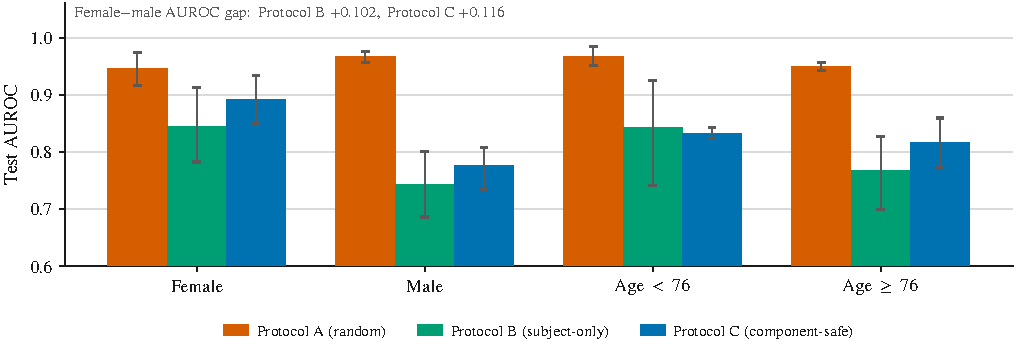
\includegraphics[width=0.95\linewidth]{figS1_subgroup_auroc.pdf}
\caption{ADNI per-subgroup test AUROC across five seeds (paired-seed
bootstrap intervals, $B=10{,}000$; descriptive). Both honest
protocols show a $\sim +0.11$ female-male AUROC gap; under the leaky
protocol the same contrast has a point estimate near zero. Reported
as exploratory, pending
external-cohort replication.}
\label{fig:adni_subgroup}
\end{figure}


% ═══════════════════════════════════════════════════════════════════════════
\section{Related work: what each prior treatment of leakage measures}
% ═══════════════════════════════════════════════════════════════════════════

Table~\ref{tab:related_work} places this work against prior treatments of leakage in AD MRI along the five axes the main text uses: whether inflation is shown, whether a dose is measured, whether provenance is varied, whether damage is observed rather than simulated, and whether split manifests are released.

\begin{table}[!ht]
\centering
\footnotesize
\caption{What prior leakage studies establish, and what this paper
adds. ``Dose'' is a measured relationship between the amount of
contamination and the reported score, rather than a comparison of two
endpoints. ``Provenance'' is whether the identifiers a protocol needs
are treated as a variable rather than assumed.}
\label{tab:related_work}
\setlength{\tabcolsep}{4pt}
\begin{tabular}{@{}lccccc@{}}
\toprule
 & Inflation & Dose & Provenance & Observed & Split \\
 & shown & measured & varied & damage & manifests \\
\midrule
Wen \etal~\cite{wen2020} (review)      & \checkmark & -- & -- & -- & -- \\
Yagis \etal~\cite{yagis2021}           & \checkmark & -- & -- & -- & -- \\
Rumala~\cite{rumala2023}                & \checkmark & -- & -- & -- & -- \\
Rosenblatt \etal~\cite{rosenblatt2024}  & \checkmark & three levels & -- & -- & -- \\
Ghiasi \etal~\cite{ghiasi2026}          & \checkmark & -- & -- & -- & \checkmark \\
DataSAIL~\cite{datasail2025} (tool)     & -- & -- & -- & -- & \checkmark \\
\midrule
This paper                              & \checkmark & continuous & \checkmark & \checkmark & \checkmark \\
\bottomrule
\end{tabular}
\end{table}

% ═══════════════════════════════════════════════════════════════════════════
\section{Which leakage-graph edge rules fire, per cohort}
% ═══════════════════════════════════════════════════════════════════════════

Table~\ref{tab:edge_provenance} counts, per cohort, how often each edge rule fires and whether it is load-bearing, meaning it merges a pair no other rule had already merged. On the two cohorts with intact identifiers every non-subject rule is redundant; \S\ref{sm:mixed_effects} is unaffected, but the provenance-degradation experiment in the main text exists precisely because that redundancy disappears when identifiers decay.

\begin{table}[!ht]
\centering
\footnotesize
\caption{Which edge rules actually fire, per dataset, counted from the
released graph-audit artefacts. The final column is the one that matters
for interpreting the component layer: an edge is \emph{load-bearing} only
if it merges a pair that no other rule had already merged. On ADNI the
session, series-UID and acquisition-date rules fire on
$223$, $209$ and $222$ pairs respectively, yet every resulting component
still contains exactly one subject, so each of those edges joined a
pair that \texttt{same\_subject} had already joined. They are redundant
on these cohorts rather than inert, and become load-bearing only where
subject identity is absent, corrupted, or inferred wrongly.
\S\ref{sec:provenance_degradation} tests that claim directly by
deleting subject identifiers at controlled rates.}
\label{tab:edge_provenance}
\setlength{\tabcolsep}{4pt}
\begin{tabular}{@{}l>{\raggedright\arraybackslash}p{5.4cm}r>{\raggedright\arraybackslash}p{5.2cm}@{}}
\toprule
Dataset & Edge rule & Pairs joined & Load-bearing here? \\
\midrule
ADNI1  & \texttt{same\_subject}     & 1{,}800 & Yes (sole component-forming rule) \\
ADNI1  & \texttt{same\_session}     & 223 & No (subsumed by subject) \\
ADNI1  & \texttt{same\_series\_uid} (source volume) & 209 & No (subsumed by subject) \\
ADNI1  & \texttt{same\_acq\_date}   & 222 & No (subsumed by subject) \\
\multicolumn{4}{@{}p{\linewidth}@{}}{\footnotesize $267/382$ ADNI components are formed by \texttt{same\_subject} alone; in the other $115$ the redundant rules also fire.} \\
\midrule
Kaggle & \texttt{same\_subject} (filename-inferred) & 6{,}076 & Fires, but the key is not participant identity \\
Kaggle & \texttt{exact\_sha256\_duplicate} & 0 & No pairs found \\
Kaggle & near-duplicate (dHash $\leq 4$) & 1{,}582 & Not merged (\textsc{review} policy) \\
\midrule
OASIS-1 & \texttt{same\_subject} & all 416 components & Yes \\
OASIS-1 & \texttt{same\_session} & all 416 components & No (subsumed by subject) \\
OASIS-1 & \texttt{same\_source\_volume} & all 416 components & No (subsumed by subject) \\
\bottomrule
\end{tabular}
\end{table}

% ═══════════════════════════════════════════════════════════════════════════
\section{Audit gate: blocking, reported and specified-but-unenforced checks}
% ═══════════════════════════════════════════════════════════════════════════

Table~\ref{tab:go_nogo} separates what the released gate enforces from what it reports and from what the framework specifies but does not yet enforce. The distinction matters because an audit whose advertised criteria exceed its implemented criteria is itself an evaluation-integrity failure.

\begin{table}[!ht]
\centering
\footnotesize
\caption{GO/NO-GO decision criteria of the released \SGA{} audit
(\texttt{scripts/audit\_adni\_splits.py}). We distinguish what the
released gate \emph{enforces} from what it \emph{reports} and from what
the framework specifies but does not yet enforce, because a leakage
audit whose advertised criteria exceed its implemented criteria is
itself an evaluation-integrity failure. Only the three blocking
checks determine the binary decision; every other quantity is written
to the audit report for author and reviewer judgement without halting
the pipeline. The gate certifies partition disjointness of the split
manifest, \emph{not} site-generalisability, scanner-shift robustness,
calibration, fairness, or clinical deployment readiness.}
\label{tab:go_nogo}
\setlength{\tabcolsep}{4pt}
\begin{tabular}{>{\raggedright\arraybackslash}p{3.9cm}>{\raggedright\arraybackslash}p{2.1cm}>{\raggedright\arraybackslash}p{5.8cm}}
\toprule
\textbf{Check} & \textbf{Status in v1} & \textbf{Behaviour} \\
\midrule
Subject overlap across partitions & \textbf{Blocking} & Any non-blank subject ID in $>1$ partition sets \texttt{passed=False}; blank and \texttt{unknown} IDs are skipped, so a cohort without identifiers cannot pass by vacuity. \\
Session overlap across partitions & \textbf{Blocking} & Any session ID in $>1$ partition sets \texttt{passed=False}. \\
Component overlap across partitions & \textbf{Blocking} & Any component ID in $>1$ partition sets \texttt{passed=False}. \\
\midrule
Per-partition label balance & Reported & Class counts and ratios written to the report. \\
Scanner field-strength balance & Reported & Marginal distribution per partition. \\
Age and sex summaries & Reported & Per-partition demographic summary. \\
Site--label association (Cram\'{e}r's $V$) & Reported & Computed by a separate script (\S\ref{sec:exp6_adni}); not consulted by the gate. \\
Component-size balance across partitions & Reported & Per-partition component-size distribution, with a warning when partitions are not drawn from comparable participants. Added after auditing this project's own frozen splits, on which it fires (\S\ref{sec:limitations}); not consulted by the gate. \\
\midrule
Unresolved subject or diagnosis identifiers & \textbf{Not enforced in v1} & No check exists. Two ADNI scans with unresolved visit-level diagnosis passed the gate for this reason (\S\ref{sec:data_adni}). \\
Frozen-manifest hash verification & \textbf{Not enforced in v1} & Hashed manifests are produced for release but the gate does not re-verify them. \\
Residual near-duplicate cross-split & \textbf{Not enforced in v1} & Near-duplicate edges are applied when \emph{building} components, not re-checked after partitioning. \\
Within-component label agreement & \textbf{Not enforced in v1} & Mixed-label converter components are handled by an explicit pre-specified exclusion rule (\S\ref{sec:data_adni}) rather than by the gate. \\
\bottomrule
\end{tabular}
\end{table}

% ═══════════════════════════════════════════════════════════════════════════
\section{Site and scanner association with label, per partition}
% ═══════════════════════════════════════════════════════════════════════════

Table~\ref{tab:site_scanner_confound_audit} reports the per-partition association between each audited covariate and the CN/AD label. The audit surfaces the confound; \SGA{} does not attempt to remove it, and the main text states why.

\begin{table}[!ht]
\centering
\footnotesize
\caption{Site and sex confound audit on the five ADNI primary-arm
component-safe splits ($1{,}125$ manifest rows, $1{,}123$
diagnosis-resolved; CN/AD rows only).
Bias-corrected Cram\'{e}r's $V$ (Bergsma~\cite{bergsma2013}) between each covariate
and the binary CN/AD label per partition; mean and range across the
five seeds. The site--label association is substantial in every
partition and grows as the partition shrinks; it is \emph{exposed}
by the audit but not \emph{resolved} by the component-safe split,
which is the central caveat of \S\ref{sec:limitations}. The
sex--label association is negligible in train and test but reaches
$V=0.34$ in the small validation partition, an instability we
attribute to its size ($n=165$) rather than to a population effect.
Scanner field strength is constant ($1.5$\,T) across every partition
of this cohort, so $V(\text{scanner}|\text{label})=0$ by
construction and the covariate is not tabulated.}
\label{tab:site_scanner_confound_audit}
\begin{tabular}{@{}lccc c@{}}
\toprule
Partition & Rows (mean) & Unique sites (range) &
$V(\text{site}|\text{label})$ (mean [min--max]) &
$V(\text{sex}|\text{label})$ \\
\midrule
Train & 793 & 38--39 & 0.360 [0.347--0.375] & 0.000 \\
Val   & 165 & 8--10  & 0.479 [0.464--0.495] & 0.343 \\
Test  & 165 & 11--12 & 0.538 [0.418--0.715] & 0.046 \\
\bottomrule
\multicolumn{5}{l}{\footnotesize
Scanner field strength is constant ($1.5$\,T) in every partition;
$V(\text{scanner}|\text{label})=0$ throughout.}
\end{tabular}
\end{table}

% ═══════════════════════════════════════════════════════════════════════════
\section{Test-partition composition under the three protocols}
% ═══════════════════════════════════════════════════════════════════════════

Table~\ref{tab:test_composition} gives the number of distinct participants, images and images per participant in each protocol's test partition. The three hold image count roughly constant while differing fourfold in how many participants those images come from, which is the asymmetry every protocol-to-protocol comparison in the main text is conditioned on.

\begin{table}[!ht]
\centering
\small
\caption{Test-partition composition per protocol on the ADNI
converter-inclusive arm (five-seed means), the arm on which the
subject-level aggregation is computed. The three protocols hold image count roughly constant
but differ fourfold in how many distinct participants those images come
from, because tightening the split rule packs more scans of fewer people
into the test partition. Every protocol-to-protocol AUROC comparison in
this paper is conditioned on this asymmetry, and we report it here rather
than leaving it implicit.}
\label{tab:test_composition}
\begin{tabular}{@{}lrrr@{}}
\toprule
\textbf{Protocol} & \textbf{Test participants} & \textbf{Test images}
                  & \textbf{Images per participant} \\
\midrule
A (random)         & $160.8$ & $213.0$ & $1.32$ \\
B (subject-only)   & $48.0$  & $220.0$ & $4.58$ \\
C (component-safe) & $38.0$  & $203.2$ & $5.35$ \\
\bottomrule
\end{tabular}
\end{table}

\bibliographystyle{unsrt}
\bibliography{references}

\end{document}
